\documentclass[10pt,twocolumn,letterpaper]{article}

\usepackage{cvpr}
\usepackage{times}
\usepackage{epsfig}
\usepackage{graphicx}
\usepackage{amsmath}
\usepackage{amssymb}
\usepackage{amsfonts}
\usepackage{multirow}
\usepackage{makecell}

\lefthyphenmin3
\righthyphenmin3
\newcommand{\app}{\raise.17ex\hbox{$\scriptstyle\sim$}}
% Include other packages here, before hyperref.

% If you comment hyperref and then uncomment it, you should delete
% egpaper.aux before re-running latex.  (Or just hit 'q' on the first latex
% run, let it finish, and you should be clear).
\usepackage[breaklinks=true,bookmarks=false]{hyperref}

%\cvprfinalcopy % *** Uncomment this line for the final submission

\def\cvprPaperID{4192} % *** Enter the CVPR Paper ID here
\def\httilde{\mbox{\tt\raisebox{-.5ex}{\symbol{126}}}}

% Pages are numbered in submission mode, and unnumbered in camera-ready
%\ifcvprfinal\pagestyle{empty}\fi
\setcounter{page}{1}
\begin{document}

%%%%%%%%% TITLE
\title{Paying More Attention to Motion: \\ Attention Distillation for Learning Video Representations}

\author{First Author\\
Institution1\\
Institution1 address\\
{\tt\small firstauthor@i1.org}
% For a paper whose authors are all at the same institution,
% omit the following lines up until the closing ``}''.
% Additional authors and addresses can be added with ``\and'',
% just like the second author.
% To save space, use either the email address or home page, not both
\and
Second Author\\
Institution2\\
First line of institution2 address\\
{\tt\small secondauthor@i2.org}
}

\maketitle
%\thispagestyle{empty}

%%%%%%%%% ABSTRACT
\begin{abstract}
We address the challenging problem of learning motion representations using deep models for video recognition. Our goal is to bridge the gap between a single RGB stream and its two stream version that uses additional flow maps as inputs. To this end, we make use of attention modules. These modules learn to highlight regions in the video and aggregate their features for recognition. Importantly, we propose to leverage their output attention maps as a vehicle to transfer the learned representations from a motion (flow) network to a RGB network. We systematically study the design of the attention module, and develop a novel attention distillation method. Our method is evaluated on major video benchmarks, and can consistently improve the performance of a base RGB network by a significant margin. Moreover, we demonstrate that the learned attention maps identify the location of actions and point out issues for feature learning. We believe our method provides a step forward towards learning to encode motion using deep models. 

%We propose a novel Attention Transfer Network for video action classification. Our proposed network has a feed forward attention mechanism that can transfer temporal knowledge from motion model to appearance model. Motion-based attention, modeled by Flow stream network, is used to supervise the appearance attention of RGB stream network.We quantitatively verify that temporal information in video inputs can be incorporated in single stream appearance network via our proposed method. We evaluate our method on multiple public datasets and show performance exceeds the state-of-the-art result by {\fontseries{b}\selectfont more than} $\mathbf{0.9 \boldsymbol{\%}}$. In addition, we elaborate a novel attention mechanism design that adopts sampling to generate probabilistic attention map. We quantitatively prove that our proposed attention mechanism is better capable of indexing key visual regions in video sequence. We conduct detailed ablation study on UCF101 and HMDB51. The experiment results show that our proposed attention mechanism outperforms baseline attention mechanism by $\mathbf{0.5\boldsymbol{\%}}$.
\end{abstract}

%%%%%%%%% BODY TEXT
\section{Introduction}

Motion is the most critical cue that links an unordered set of frames into a meaningful video. Unfortunately, learning motion representations from video frames remains challenging for deep models. Recent deep networks have the capacity to capture the temporal dynamics in video frames, e.g., via 3D convolutions~\cite{tran2015learning} or recurrent architectures~\cite{donahue2015long}. However, the performance of these models using RGB video frames (RGB stream) falls far behind their two-stream versions~\cite{donahue2015long,carreira2017quo}, where motion is explicitly encoded by optical flow (flow stream). In fact, a recent study~\cite{Feichtenhofer_2018_CVPR} showed that for the same input video, the flow stream produces qualitatively different features as to the RGB stream.

Why did these models fail to learn effective motion representations from video frames? Consider the examples in Fig.\ \ref{fig:teaser}. Given the input videos, we visualize the attention maps of RGB and flow streams from state-of-the-art 3D networks for action recognition (I3D~\cite{carreira2017quo}). These maps reveal different ways of recognizing actions. RGB attention selects discriminative appearance patterns, including foreground regions of the actions or background regions of contextual cues (e.g., hula hoop). On the other hand, flow attention highlights the moving parts that characterize unique motion patterns. It seems that there is no incentive for the RGB stream to encode motion, as the appearance patterns already provide an ``easy'' route for recognition. 

\begin{figure}[t]
\centering
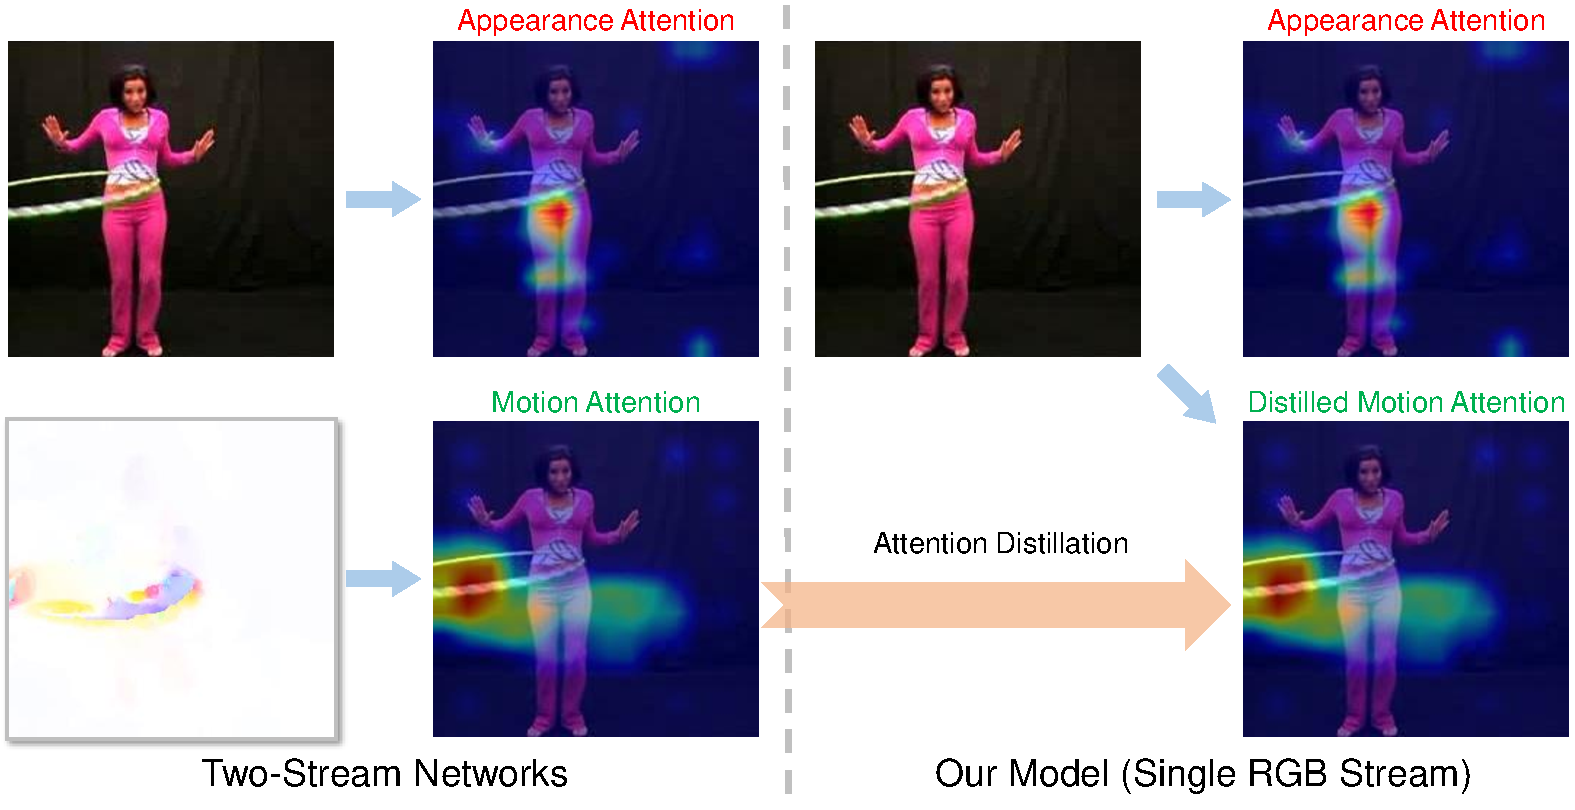
\includegraphics[width=1.0\linewidth]{latex/figures/teaser_new.pdf}
\caption{Attention maps from RGB and flow streams of I3D~\cite{carreira2017quo} computed using Grad-Cam~\cite{selvaraju2017grad}. RGB network and flow network attends to different aspects of an action, yet both are essential for recognition. We thus propose to use the attention map as the bridge to transfer knowledge from the motion stream to the RGB stream.} 
\label{fig:teaser}
\vspace{-1.2em}
\end{figure}

As a remedy to this challenge, several recent works have developed novel architectures to facilitate the learning of spatiotemporal features~\cite{Hara_2018_CVPR,Tran_2018_CVPR,Xie_2018_ECCV,Sun_2018_CVPR,fan2018end}. Our work shares the same motivation, yet pursues a vastly different approach. We seek to regularize the learning of the RGB stream by asking the RGB network to mimic the ``motion'' attention from the flow stream. By distilling attention across modalities, the RGB network is required to understand which regions are moving, and thus more likely to capture the motion patterns associated with the actions. To this end, we make use of attention mechanisms developed for image recognition~\cite{wang2017residual,Zagoruyko2017AT}, and re-purpose them for action recognition in videos. More importantly, we propose a novel attention distillation scheme that transfers temporal knowledge from the flow stream to the RGB stream. 

Specifically, our model learns to jointly predict appearance and motion attention maps. These maps are further used to independently aggregate visual features. The results are two vector representations that capture two different ``views'' of the video. These vectors are further passed through a sub-network for final classification. During training, we adopt a reference flow network with soft attention mechanism as the teacher network. And we require the motion attention of our model to match the attention of the teacher (flow) network. Moreover, we explore different approaches for learning the attention maps. In consequence, our motion attention learns to point to foreground moving regions, and our appearance attention learns to select discriminative regions for recognition. During testing, our model only needs video frames as inputs, and uses two attention maps to index visual features for recognition. 

We conduct extensive experiments to evaluate our model. To begin with, we perform a systematical study of the attention modules for action recognition. Our results suggest that a proper designed attention module can slightly improve the recognition results. By leveraging this attention module, we further evaluate our proposed attention distillation on three datasets: UCF101~\cite{Soomro2012UCF101AD}, HMDB51~\cite{kuehne2011hmdb} and 20BN-Somthing-Something-V2~\cite{goyal2017something,mahdisoltani2018fine}. Our method consistently improves the recognition accuracy by at least $1\%$ over state-of-the-art methods that only use RGB frames. However, our results still fall behind the two stream networks. We provide further analysis of learned attention and features. Our experiments shows that our motion attention maps help to localize actions, yet the features do not fully capture the concept of motion. Nonetheless, we believe that our work provide a baby step towards the challenging problem of learning spatiotemporal features from video frames. 



%------------------------------------------------------------------------
\section{Related Works}

%-------------------------------------------------------------------------
\subsection{Action Recognition}
Action recognition is a well established topic in computer vision. A recent survey can be found in~\cite{poppe2010survey}. And we focus on methods using deep models. 

Simonyan and Zisserman~\cite{simonyan2014two} proposed two-stream convolutional networks. Their key idea is to factorize the learning of spatial and temporal features into two networks--a RGB network using video frames and a flow network using optical flow maps. Spatiotemporal features can also be learned from video frames using recurrent networks. Donahua et al.\ \cite{donahue2015long} proposed to model a sequence of frames using LSTMs~\cite{hochreiter1997long}. A similar idea was discussed in~\cite{yue2015beyond}. More recently, Tran et al.\ \cite{tran2015learning} proposed to use 3D convolutional networks for action recognition. This idea was further extended by Carreira et al.\ \cite{carreira2017quo}. Their I3D model make use of two stream 3D networks for learning video representations. Both recurrent networks and 3D convolutional networks have the ability to capture motion beyond a single frame. However, their performance using video frames alone still falls far behind their two stream versions~\cite{yue2015beyond,carreira2017quo}. Our work seek to address this challenge of learning motion-aware video representations from RGB frames.  

There are several recent attempts to address this challenge. Ng et al.\ \cite{ng2016actionflownet} proposed to jointly predict action labels and flow maps based on video frames and using multi-task learning. This idea is extended by Fan et al.\ \cite{fan2018end}, where they fold the TV-L1 flow estimation into their TVNet. Without using flow, Tran et al.\ \cite{Tran_2018_CVPR} demonstrated that factorized 3D convolution (2D spatial convolution and a 1D temporal convolution) can facilitate the learning of spatiotemporal features and achieve higher recognition accuracy. A similar finding was also presented by Xie et al.\ \cite{Xie_2018_ECCV}. Our method shares the same motivation as these approaches. However, we take a different route. We did not consider learning to predict flow maps nor design novel architectures. Instead, we explored using attention mechanisms for video recognition, and proposed to distill the predicted attention to transfer knowledge from a flow network to a RGB network.
%-------------------------------------------------------------------------

%-------------------------------------------------------------------------

\subsection{Knowledge Distillation}
Our attention distillation is closely related to knowledge distillation, first proposed by Caruana et al.\ \cite{buciluǎ2006model} for model compression, and further popularized by Hinton et al.\ \cite{hinton2015distilling}. Knowledge distillation seek to match the intermediate activations or outputs between a teacher network and a student network. For example, the softmax output of a teacher network can be used as a soft target for supervising the learning of a student network~\cite{hinton2015distilling}. The most relevant work comes from Zagoruyko et al.\ \cite{Zagoruyko2017AT}. They also used attention to transfer knowledge from a teacher network to a student network. Our method shares the same intuition. We seek to transfer motion knowledge from a flow network to a RGB network, using their attention maps as the bridge. 

However, our method differs from Zagoruyko et al.\ \cite{Zagoruyko2017AT} in three key aspects. First, we use soft attention for recognition. And thus our attention maps focus on discriminative regions. This is different from the attention in~\cite{Zagoruyko2017AT}, i.e., using average/max values of the feature maps or their gradients. Second, we consider distillation between two different modalities. Matching the feature maps or their gradients from two modalities is unlikely to work. Third, we no longer assume that the teacher model is superior to the student network. In fact, in many cases, the performance of our teacher flow network is sub par to the student RGB network. Instead, our attention distillation aims at learning to encode motion from video frames. In experiment section, we carefully compare the results of our method to~\cite{Zagoruyko2017AT}.
%-------------------------------------------------------------------------

\begin{figure*}[t]
\centering
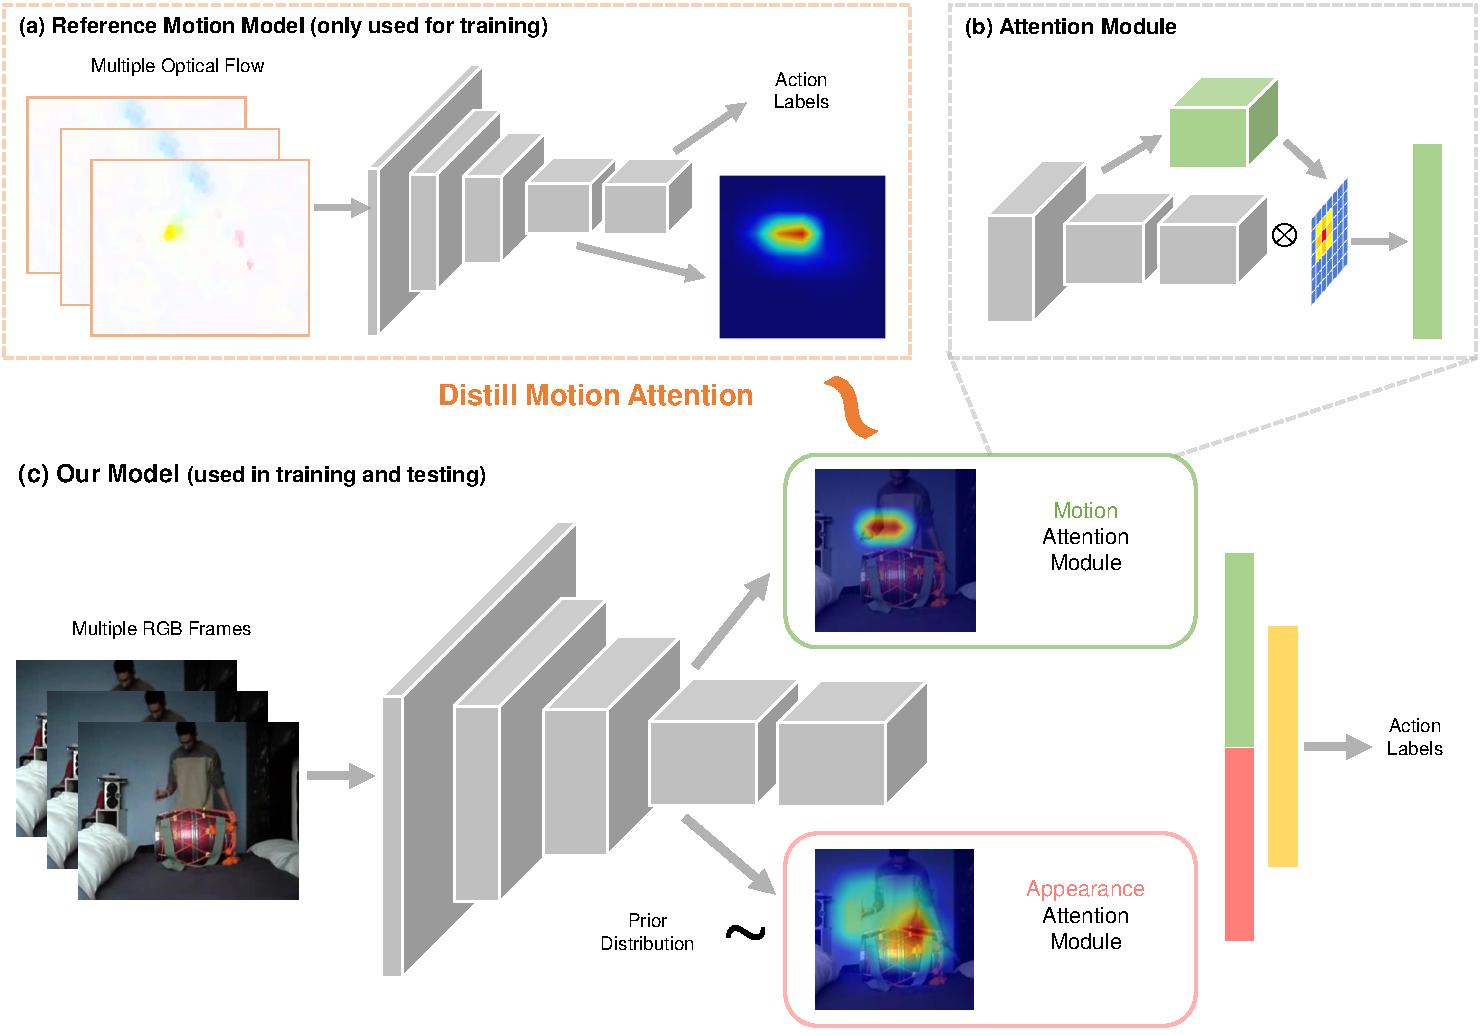
\includegraphics[width=0.8\linewidth]{figures/overview.pdf}
\caption{Overview of our method. Our method (c) takes multiple RGB frames as inputs and make use of a backbone 3D convolutional network. Our model outputs two attention maps using the attention module (b), based on which the action labels are predicted. The motion map is learned by mimicking the attention from a reference flow network (a). And the appearance map that is learned to highlight discriminative regions for recognition. These two maps are used to create motion-aware feature representations from video frames for action recognition. Our work makes two key contributions. First, we present a systematical study of attention based recognition in videos. Second, we propose to leverage attention as the vehicle to transfer knowledge between different modalities for video recognition.} 
\label{fig:flowchart}
\vspace{-1.0em}
\end{figure*}

\subsection{Attention for Recognition}
Attention has been widely used for visual recognition. Top-down task-driven attention can guide the search of objects~\cite{oliva2003top}, select local descriptors for object or action recognition~\cite{gao2009discriminant,mathe}, or localize actions~\cite{gregNIPS}. More recently, attention has been explored in deep models for object recognition~\cite{mnih2014recurrent} and image captioning~\cite{xu2015show}. Attention enables these models to ``fixate'' on image regions, where the decision is made based on a sequence of fixations. This definition is different from self-similarity as in~\cite{vaswani2017attention}. 
Several attention mechanisms are proposed for deep models. For example, Sharma et al.\ \cite{sharma2015action} integrated soft attention in LSTMs for action recognition. Li et al.\ \cite{li2018videolstm} further extends~\cite{xu2015show} into videos. Specifically, they combined LSTMs with motion-based attention to infer the location of the actions. Girdhar and Ramanan~\cite{Girdhar_17b_AttentionalPoolingAction} modeled top-down and bottom-up attention using bilinear pooling. Wang et al.\ \cite{wang2017residual} proposed a residual architecture for soft attentions. Li et al.\ \cite{Li_2018_ECCV} considered attention as a probabilistic distribution. Our method explored attention mechanisms from previous approaches for distillation. We also provide a systematical study of these methods for action recognition. 


\section{Distilling Motion Attention for Actions}
In this section, we present our method of attention distillation for action recognition. We start with an overview of the key ideas, followed by detailed description of the components in our method. Finally, we describes our network architecture and discuss implementation details.

\subsection{Overview}
For simplicity, we consider an input video with fixed length of $T$ frames. Our method can easily generalize to multiple videos, e.g., for mini-batch training. We denote the input video as $x=\{x^1, x^2, ..., x^T\}$, where $x^t$ is a frame of resolution $H\times W$ with $t$ as the frame number. Given $x$, our goal is to predict a video-level action label $y$. And we leverage the intermediate output of a 3D convolutional network $\phi$ to represent $x$. This is given by a 4D tensor $\phi(x)$ of the size $T_\phi \times H_\phi \times W_\phi \times C_\phi$. $C_\phi$ is the feature dimension of 3D tensor $T_\phi \times H_\phi \times W_\phi$ from the video $x$. Our method consists of three key components.

\noindent \textbullet\ \textbf{Attention Generation}: The model first predicts an attention map $\mathcal{A}$ based on $\phi(x)$ using attention mapping function $F_{\mathcal{A}}$. $\mathcal{A}$ is a 3D tensor of size $T_\phi \times H_\phi \times W_\phi$. Moreover, $\mathcal{A}$ is normalized within each temporal slice, i.e., $\sum_{w,h} \mathcal{A}(t,w,h)=1$. $\mathcal{A}$ is thus a sequence of 2D attention maps $\mathcal{A}(t)$ defined over $T_\phi$ steps. 

\noindent \textbullet\ \textbf{Attention Guided Recognition}: Based on the attention map $\mathcal{A}$ and the features $\phi(x)$, the model further applies a recognition module $F_{\mathcal{R}}$ that outputs the action label $y$. Specifically, this module uses $\mathcal{A}$ to selectively pool features from $\phi(x)$, followed by a classifier that maps the result feature vector to $y$.

\noindent \textbullet\ \textbf{Attention Distillation}: To regularize the learning, we assume that $\mathcal{A}$ will receive supervision from a teacher model that outputs a reference attention map $\mathcal{\tilde{A}}$. Our teacher model comes from a different modality and is equipped with the same attention mechanism for recognition.

Fig.\ \ref{fig:flowchart} presents an overview of our method. Our model takes the input of a video clip $x$, and learns to predict two attention maps based on $\phi(x)$: $\mathcal{A}^M$ for motion attention and $\mathcal{A}^A$ for appearance attention. Based on these two maps, the model further aggregates visual features that will be passed into final recognition sub-network. During training, we match $\mathcal{A}^M$ to the attention map $\mathcal{\Tilde{A}}^M$ from the reference flow network. For testing, only the input video is required for recognition. Our model also outputs two attention maps that can be used to help diagnosing the results. We now detail the design of our key components.

\subsection{Attention Generation}
We explore two different approaches for generating an attention map from the features $\phi(x)$, including soft attention~\cite{wang2017residual} and its probabilistic version~\cite{Li_2018_ECCV}.

\noindent \textbf{Soft Attention}: Attention maps can be created by a linear function of $w_a \in R^{C_\phi}$ over the feature map $\phi(x)$,
\begin{equation}
\small
    F_{\mathcal{A}}(\phi(x)) = softmax(w_a * \phi(x)),
\end{equation}
where $*$ is the convolution (1x1) on the 3D feature grids. Softmax is applied on every time slice to normalize the map.

\noindent \textbf{Probabilistic Soft Attention}: An alternative approach is to further model the distribution of linear mapping outputs as discussed in~\cite{Li_2018_ECCV}, namely 
\begin{equation}
\small
    \mathcal{A} \app p(\mathcal{A}) = softmax(w_a * \phi(x))
\end{equation}
where we model the distribution of $A$. During training, an attention map can be sampled from $p(\mathcal{A})$ using Gumbel Softmax trick~\cite{jang2016categorical, maddison2016concrete}. We follow~\cite{Li_2018_ECCV} to regularize the learning by adding additional loss term of 
\begin{equation}
\label{eq:reg_atten}
\small
    \mathcal{L}^R = \sum_t KL\left[\mathcal{A}(t) || U\right], 
\end{equation}
where $KL[\cdot]$ is the Kullback-Leibler divergence and $U$ is the 2D uniform distribution ($H_\phi \times W_\phi$). This term seek to match each time slice of the attention map to a prior distribution. It is derived from variational learning and accounts for (1) the prior of attention maps and (2) additional regularization by spatial dropout~\cite{Li_2018_ECCV}. During testing, we directly plug in $p(\mathcal{A})$ (the expected value of $\mathcal{A}$).

Note that for both approaches, we restrict $F_{\mathcal{A}}$ to a linear mapping without a bias term. In practice, this linear mapping avoids a trivial solution of generating a uniform attention map. This is because that this trivial solution can only be achieved by setting $w$ to an all-zero vector, which rarely happens during training with a proper initialization of $w$.

\subsection{Attention Guided Recognition}
Our recognition module makes use of an attention map $\mathcal{A}$ to select features from $\phi(x)$. Again, we consider two different models for the attention guided recognition. 

\noindent \textbf{Attention Pooling}: We follow the attention mechanism in~\cite{wang2017residual,liu2018end} and design the function $F_{\mathcal{R}}$ as 
\begin{equation}
\label{eq:direct_atten}
\small
    \Tilde{y} = F_{\mathcal{R}}(\phi(x), \mathcal{A}) = softmax\left( W_r^T (\mathcal{A} \otimes \phi(x)) \right)
\end{equation}
where $\otimes$ denotes the tilted multiplication $\mathcal{A} \otimes \phi(x) = \sum_{t,h,w} \mathcal{A}(t, h, w) \phi(x)_{t,h,w,c}$. The module is equivalent to weighted average pooling over $\phi(x)$, followed by linear classifiers $W_r$ with softmax normalization. Specifically, the weights used for pooling ($\mathcal{A}$) are shared across all channels.
 
\noindent \textbf{Residual Connection}: Using the attention map to re-weight features helps to filter out background noises, yet may also raise potential danger of missing important foregrounds. This drawback was discussed in~\cite{wang2017residual} and we follow their solution of adding a residual connection to the attention map. This is given by 
\begin{equation}
\label{eq:res_atten}
\small
    \Tilde{y} = F_{\mathcal{R}}(\phi(x), \mathcal{A}) = softmax\left( W_r^T ( (\mathcal{A}+I) \otimes \phi(x) ) \right)
\end{equation}
where $I$ is a 3D tensor of all ones. Intuitively, this module further adds an average pooled features to the vector before the linear classifier. By adding the residual term, features learned by the network are preserved. 

\subsection{Attention Distillation}
The key of our method lies in the attention distillation during training. Specifically, we assume a reference flow network is given as the teacher network. The teacher model also uses attention mechanism for recognition. And its motion attention map $\mathcal{\Tilde{A}}^M$ is used as additional supervisory signal for training our RGB network. This RGB network is thus the student model that mimics the motion attention map. With probabilistic attention modeling, the imitation of the attention maps is enforced by using the loss
\begin{equation}
\label{eq:distill}
\small 
    \mathcal{L}^{\mathcal{A}} = \sum_t\  KL\left[ \mathcal{A}^M(t)||\mathcal{\Tilde{A}}^M(t) \right].
\end{equation}
This loss minimizes the distance between the attention maps at every time step $t$. In practice, our teacher flow network is pre-trained with the same attention mechanism. Once trained, the weights of teacher model remains fixed during the learning of the student model. And only the student model (RGB network) is used for inference. 

\subsection{Our Full Model}
Putting everything together, we summarize our full model with probabilistic soft attention and attention distillation. Specifically, our model estimate two probabilistic attention maps of $p(\mathcal{A}^M) \sim F_{\mathcal{A}}^M(\phi(x))$ (motion) and $p(\mathcal{A}^A) \sim F_{\mathcal{A}}^A(\phi(x))$ (appearance). These maps are further used to predict the action labels. This is given by 
\begin{equation}
\small
    \Tilde{y} = F_{\mathcal{R}}^M(\phi(x), p(\mathcal{A}^M)) + F_{\mathcal{R}}^A(\phi(x), p(\mathcal{A}^A))
\end{equation}
where each $F_{\mathcal{R}}$ follows Eq~\ref{eq:res_atten}.

\noindent \textbf{Loss Function}: Our training loss is defined as
\begin{equation}
\small
\begin{split}
    \mathcal{L} = CE(\Tilde{y}, y) &+ \lambda_1 \sum_t\  KL\left[ \mathcal{A}^M(t)||\mathcal{\Tilde{A}}^M(t) \right] \\
                  & + \lambda_2 \sum_t KL\left[ \mathcal{A}^A(t)||U \right],
\end{split}
\end{equation}
where $CE$ is the cross entropy loss between the predicated labels $\Tilde{y}$ and the ground-truth $y$. Thus, the loss consists of three terms. The first cross entropy term is to minimize the error for classification. The second KL term (from Eq.\ \ref{eq:distill}) enforces that the motion attention $\mathcal{A}^M$ mimic the attention map $\mathcal{\Tilde{A}}^M$ from the reference flow network. And the third KL term (from Eq.\ \ref{eq:reg_atten}) regularizes the learning of the appearance attention. The coefficients $\lambda_1$ and $\lambda_2$ are used to balance the three terms. We choose $\lambda_{i}$ as $\tau^2/ (T_\mathcal{A}\times W_\mathcal{A}\times H_\mathcal{A})$, where $1/ (T_\mathcal{A}\times W_\mathcal{A}\times H_\mathcal{A})$ is a normalizer. 


\subsection{Implementation Details}
\noindent \textbf{Network Architecture}: 
Our model makes use of I3D model~\cite{carreira2017quo} as the backbone network. Specifically, I3D has five 3D convolution blocks, and three of them are composed of multiple Inception Modules. For all attention module, intermediate feature $\phi$ is obtained from the final Inception Module of the 4th convolution block. The attention map is used to select the final network feature from the last Inception module of the 5th block.

\noindent \textbf{Data Preparation}:
We downsample all frames to $320\times256$ and maintain a frame rate of 24. For training, we calculate optical flow using TV-L1~\cite{perez2013tv}. We adopt several data augmentations, including random flipping, cropping and color jittering to prevent overfitting. Our model takes 24 consecutive frames as inputs. All input frames are cropped to $224\times224$ for training. During inference time, we test our model on full resolution video clips ($320\times256$). We aggregate scores from all clips to produce the video-level results.

\noindent \textbf{Training Details}:
All our models are trained using SGD with momentum of 0.9. Their weights are initialized from Kinetics pre-trained model provided by the authors of~\cite{carreira2017quo}. We train the models with a batch size of 64 on 4 GPUs. The initial learning rate is 0.01 with a decay rate of 10 when loss starts to saturate. Our model use both batch norm and weights decay (0.9 decay rate). We apply dropout on the output of final average pooling layer before recognition network with dropout rate 0.7. Our model is implemented in Tensorflow and the code will be made public available.

\section{Experiments}
We now present our experiments and results. Our results are summarized into three parts. First, we provide a systematical evaluation of attention guided action recognition. Second, we benchmark our attention distillation and compare our results to the state-of-the-art methods on several public datasets. Finally, we further investigate what have been learned by our model. We show that (1) our predicted attention maps help to localize actions in the video; and (2) our model is better at capturing the concept of motion in comparison to a vanilla RGB network.  

\subsection{Attention Guided Action Recognition}
We start from an ablation study of attention guided action recognition. Specifically, we evaluate different combinations of attention generation and attention based recognition. And we compare their results to those from models without attention. Our experiments shows that a proper design of the attention mechanism can consistently improve the performance of action recognition across datasets. We now present our benchmark, baselines and results. 

\noindent \textbf{Benchmark}: We use two public action recognition datasets for this experiment: UCF101 and HMDB51. UCF101~\cite{Soomro2012UCF101AD} contains 13,320 videos from 101 action categories. And HMDB51~\cite{kuehne2011hmdb} includes 6,766 videos from 51 action categories. We evalute mean class accuracy and report the results using the first split of these two datasets. 

\begin{table}[t]
\footnotesize
\centering
\begin{tabular}{c|c|cc}
\multicolumn{2}{c|}{\multirow{2}{*}{Method}}                                                      & \multicolumn{2}{c}{Mean Class Accuracy} \\
\multicolumn{2}{c|}{}                                                                              & UCF101        & HMDB51        \\ \hline 
\multirow{5}{*}{RGB Stream}                                               
                                                                           & \makecell{I3D (backbone)}  & 94.8              & 70.9  \\
                                                                           & \makecell{Soft-Atten}      & 94.7              & 70.8      \\
                                                                           & \makecell{Soft-Res}        & 94.9              & 70.1              \\
                                                                           %& \makecell{Prob-Atten-noreg}      & 94.8              & 71.1         \\ % This is P
                                                                  
\multirow{7}{*}{\begin{tabular}[c]{@{}c@{}}Flow Stream\end{tabular}}       & \makecell{Prob-Atten}        & \textbf{95.1}     & \textbf{71.3}             \\ 
\hline
                                                                           & \makecell{I3D (backbone)}  & 94.0              & 73.9              \\
                                                                           & \makecell{Soft-Atten}      & 94.7              & 74.1              \\
                                                                           & \makecell{Soft-Res}        & \textbf{95.2}     & \textbf{74.4}            \\													                       
                                                                           %& \makecell{Prob-Atten-noreg}      & 94.7              & 74.1              \\                                        
                                                                           & \makecell{Prob-Atten}        & 94.9              & 74.2            \\
\end{tabular}
\vspace{0.1em}
\caption{Evaluation of the attention modules. We compared 3 different design choices with RGB and flow streams on UCF101 and HMDB51. Adding attention to the backbone I3D marginally improves the RGB stream ($0.3\%-0.4\%$) and slightly boost the performance of flow stream ($0.5\%-1.2\%$). Prob-Atten provides consistent performance boost on both streams and across datasets.}
\label{table:ablation}
\end{table}

\noindent \textbf{Baselines}: We consider the different combinations of how the model generate attention maps (Soft vs. Probabilistic Attention) and how the attention maps are used for recognition (Attention Pooling vs. Residual Connection). The valid combinations include\\
\textbullet\ \textbf{Soft-Atten} is a standard attention module (e.g., used in~\cite{liu2018end}) that combines the soft attention and the attention pooling for recognition.\\
\textbullet\ \textbf{Soft-Res} is the residual attention module in~\cite{wang2017residual} that further adds residual connection to Soft-Atten. \\
\textbullet\ \textbf{Prob-Atten} is the probabilistic attention module in~\cite{Li_2018_ECCV} that combines probabilistic modeling of attention with the attention pooling.

Note that the combination of Prob+Res is not valid as it violates the probabilistic modeling of attention. In practice, we found its training unstable. Therefore, we report the results of three valid designs for both RGB and flow stream on UCF101 and HMDB51 datasets. We also include results of the vanilla I3D models (our backbone) using the same input sequence length (24 frames) as our methods. These results are summarized in Table~\ref{table:ablation}.

\noindent \textbf{Results}: Adding attention to the backbone recognition network almost always improves the performance by a small margin, with the exception of the Soft-Atten. This is probably because vanilla soft attention has the drawback of omitting too much information. The performance boost from the attention module is larger for the flow stream in comparison to the RGB stream. For both UCF101 and HMDB51, the best performing method is Prob-Atten for RGB stream (+$0.3\%/0.4\%$) and Soft-Res for flow stream (+$1.2\%/0.5\%$). Prob-Atten also outperforms the I3D baseline for flow stream, yet Soft-Res decrease the performance of RGB stream on HMDB51. Across the modalities and datasets, Prob-Atten is the only design that can consistently improve the recognition accuracy. This boost might be explained by the additional regularization posed by the sampling. Therefore, we choose Prob-Atten as our attention module for both the reference flow network and our RGB network in the rest of our experiments. 


\subsection{Attention Distillation for Action Recognition}

We now evaluate our model with attention distillation. In this setting, we assume a reference flow network with attention module is given at training time. We attach two attention modules to our RGB backbone. The appearance attention follows the standard probabilistic attention module. And the flow attention is asked to mimic the attention map from reference flow network. We present our benchmark and results on action recognition, and contrast our method with a relevant work on attention transfer~\cite{Zagoruyko2017AT}.  

\noindent \textbf{Benchmark}: We compare our results on action recognition with state-of-the-art methods on UCF101 and HMDB51. Again, we report mean class accuracy on these two dataset. Moreover, we experimented with a large scale video dataset: 20BN Something-Something-v2 (20BN-V2)~\cite{mahdisoltani2018fine}. This new dataset has over 220K videos and 174 fine-grained action categories. The action labels of 20BN-V2 follows a long-tailed distribution, making the dataset very challenging. We follow their data splits. Our model is trained on the training set, and tested on their validation set. We report top-1 and top-5 accuracy following~\cite{mahdisoltani2018fine,zhou2017temporal} and compare our results to a strong set of baselines.

\begin{table}[t]
\footnotesize
\centering
\begin{tabular}{c|c|cc}
\multicolumn{2}{c|}{\multirow{2}{*}{Method}}                                                      & \multicolumn{2}{c}{Mean Class Accuracy} \\
\multicolumn{2}{c|}{}                                                                              
& UCF101        & HMDB51        \\ \hline 
\multirow{5}{*}{RGB + Flow}                                              
& \makecell{Two Stream~\cite{simonyan2014two}  }                        & 88.0              & 59.4      \\
& \makecell{Two Stream LSTM~\cite{yue2015beyond}  }                     & 88.6              & $-$      \\
& \makecell{Joint Two stream~\cite{feichtenhofer2016convolutional}  }   & 92.5              & 65.4        \\
& \makecell{TSN~\cite{wang2016temporal}}                                & 94.0              & 68.5             \\                                           
\multirow{11}{*}{\begin{tabular}[c]{@{}c@{}}RGB Only\end{tabular}}      
& \makecell{Two Stream I3D~\cite{carreira2017quo} }                     & 96.8\text{*}      & 76.1\text{*}             \\ 
\hline
& \makecell{VGG16~\cite{simonyan2014two} }                              & 73.0              & 40.5              \\
& \makecell{RGB LSTM~\cite{yue2015beyond}  }                            & 82.6              & $-$      \\
& \makecell{RGB TSN~\cite{wang2016temporal}}                            & 84.5              & $-$           \\
& \makecell{C3D~\cite{tran2015learning} }                               & 82.3              & $-$              \\
& \makecell{P3D ResNet~\cite{qiu2017learning}  }                        & 88.6              & $-$      \\
& \makecell{ActionFlowNet~\cite{ng2016actionflownet}}                   & 83.9              & 56.4            \\	
& \makecell{TVNet~\cite{fan2018end} }                                   & 94.5              & 71.0              \\    
& \makecell{I3D RGB (backbone)~\cite{carreira2017quo} }                 & 94.8\text{*}      & 70.9\text{*}            \\
& \makecell{Ours (RGB)}                                                 & \textbf{95.7}     & \textbf{72.0}            \\
\hline
\multirow{2}{*}{\begin{tabular}[c]{@{}c@{}}64 Frames RGB\end{tabular}}  
& \makecell{I3D RGB ~\cite{carreira2017quo} }                           & 95.6              & 74.8          \\
& \makecell{S3D~\cite{Xie_2018_ECCV}}                                   & 96.8              & 75.9            \\
\end{tabular}
\vspace{0.1em}
\caption{Results of action recognition on UCF101 and HMDB51. We compare the results of our model with several previous methods. Our model outperforms state-of-the-art results that use single RGB stream by $\app 1\%$. \text{*}For fair comparison, we report results of I3D models that use 24 frames as inputs--the same as our model.}
\label{table:action}
\end{table}

\begin{table}[h]
\centering
\footnotesize
\begin{tabular}{c|cc}
Method                                 & Top-1/5 Acc  & Temporal Footprint  \\ \hline 
TRN RGB~\cite{zhou2017temporal}        & 48.8 / 77.6      & 5 sec        \\
TRN RGB+Flow~\cite{zhou2017temporal}   & 55.5 / 83.1      & 5 sec        \\ \hline
I3D RGB+Atten (backbone)               & 48.1 / 78.8      & 1 sec     \\
I3D Flow+Atten (ref)                   & 48.3 / 78.9      & 1 sec      \\ 
Ours (RGB)                             & 49.4 / 79.5      & 1 sec        \\
%Two-stream I3D + Attention      & 53.5   & 1s        \\
\end{tabular}
\vspace{0.1em}
\caption{Action recognition results on on 20BN-V2 dataset~\cite{mahdisoltani2018fine}. We report top-1/top-5 accuracy and the temporal footprint of the inputs. Our results are compared against a set of baselines. Again, our model achieves the best performance among networks that uses RGB frames, yet falls behind the two stream networks that use both frames and flow maps.}
\label{table:20bn}
\end{table}

\noindent \textbf{Results}: Our results on UCF101 and HMDB51 datasets are presented in Table~\ref{table:action}. These results are grouped based on the modalities they used (RGB+flow vs.\ RGB) and the sequence length they used. It worth noting that several works~\cite{carreira2017quo,Xie_2018_ECCV} achieved superior performance, yet they adopt a much longer sequence length (64 frames). For fair comparison, we only benchmark our result with models that use less than 24 frames. And our model uses RGB frames for recognition, yet distills attention from a reference flow network. Our method reaches a mean class accuracy of $95.7\%$ on UCF101 and $72.0\%$ on HMDB51. Our results outperform all previous methods that using only RGB frames with sequence length smaller than 25 frames.  Specifically, our results are +$1.2\%$ better than our direct competitors that seek to learn motion representations from video frames, e.g., ActionFlowNet~\cite{ng2016actionflownet} and TVNet~\cite{fan2018end}. Part of this performance boost is because of our strong backbone RGB network (I3D). However, our model further improves our backbone by $0.9\%$ on UCF101 and $1.1\%$ on HMDB51. And this improvement provides a solid support of our attention distillation idea. We have to point out that our result still lags behind the two stream network (Two Stream I3D). Our model is -$1.1\%$ worse on UCF101 and -$4.1\%$ on HMDB51. This gap suggests that our model does not fully capture the concept of motion that is encoded in two stream networks. Nonetheless, we beleive that our model provide a key step forward for learning to encode motion from RGB frames. 

Moreover, we report results of our method on 20BN-V2 in Table~\ref{table:20bn}. Even with 1/5 of the temporal receptive field as to the latest TRN~\cite{zhou2017temporal}, our model with RGB frames outperform the TRN RGB by $0.6\%/1.9\%$ in top-1 and top-5 accuracy . In fact, our backbone network (I3D RGB) has slightly worse performance than TRN. And our method improves the backbone by $1.3\%$ in top-1 and $0.7\%$ in top-5. Our model with RGB frames also outperform the reference flow network used for attention distillation by $1.1\%$ in top-1 and $0.6\%$ in top-5. Again, our results are lagging behind the two stream networks. The ranking of results remains consistent as those on UCF101 and HMDB51.

\begin{table}[t]
\centering
\footnotesize
\begin{tabular}{c|cc}
\multirow{2}{*}{Method}                        & \multicolumn{2}{c}{Mean Class Accuracy} \\
                                               & UCF101   & HMDB51 \\ \hline
I3D RGB (backbone)                             & 94.8     & 70.9   \\
ActivationMax~\cite{Zagoruyko2017AT}           & 94.3     & 70.7   \\
%Soft-Atten (Ours) & 95.0 & 70.8       \\ 
Ours                                           & 95.7     & 72.0   \\ 
\end{tabular}
\vspace{0.1em}
\caption{Comparison between our attention distillation and attention transfer in~\cite{Zagoruyko2017AT}. Matching the feature activation across modalities decreases the mean class accuracy.}
\label{table:transfer}
\end{table}

\begin{figure*}[t]
\centering
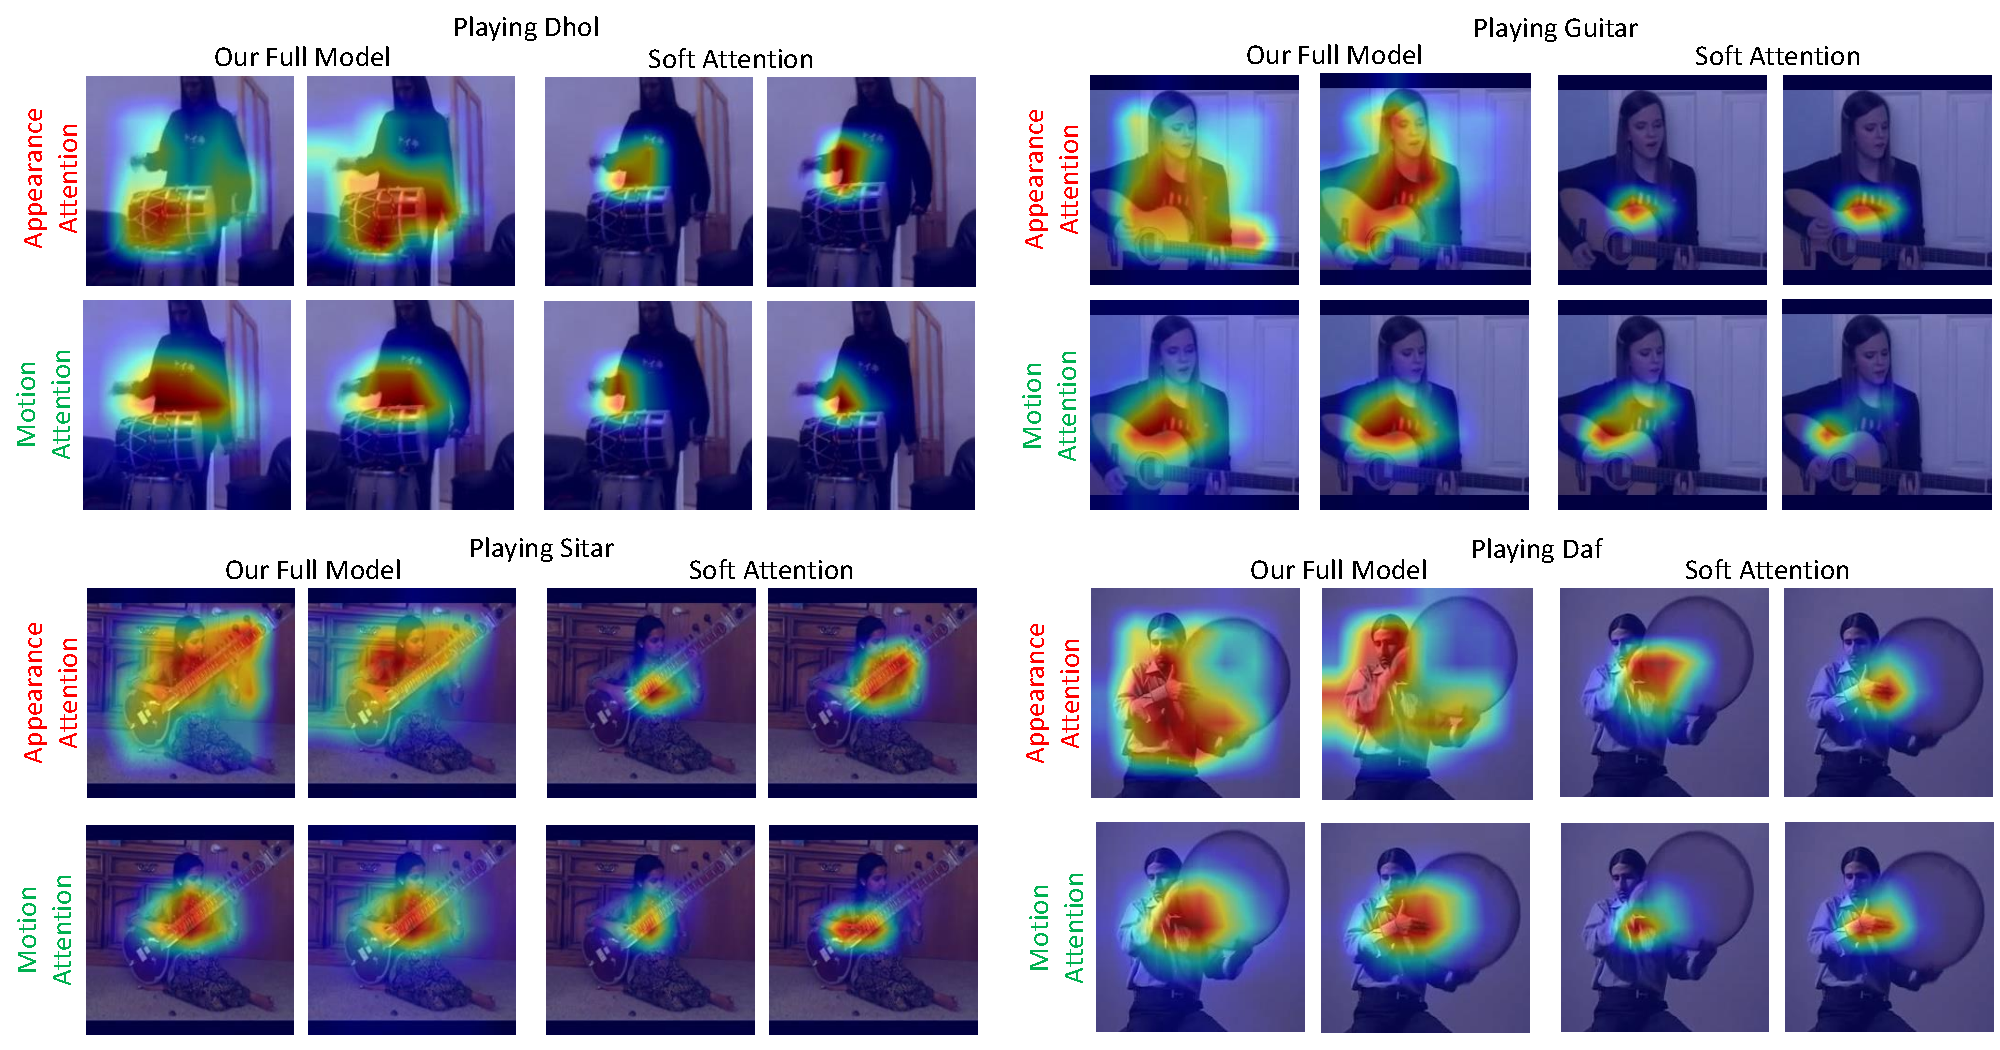
\includegraphics[width=0.9\linewidth]{figures/vis.pdf}
\caption{Visualization of attention maps from our method and base networks. For each video clip, we re-interpolate the attention maps and plot them on the first and last frame. Red regions indicate higher value of attention. Our model produces qualitatively different appearance and motion attention, which seem to index key regions of actions.}
\label{fig:vis}
\vspace{-1em}
\end{figure*}

\noindent \textbf{Comparison to Attention Transfer~\cite{Zagoruyko2017AT}}: We further contrast our model with the related work of attention transfer in~\cite{Zagoruyko2017AT}. The key differences between our model and~\cite{Zagoruyko2017AT} are the definition of attention and the transfer of attention cross modalities. To this end, we conduct further experiment to highlight the performance gap produced by these differences. Concretely, we implement~\cite{Zagoruyko2017AT} on our backbone network (I3D RGB). In addition to the classification task, this RGB network (ActivationMax) is trained to mimic the ``attention'' from the flow network. While the idea sounds similar, the attention is defined as the maximum activation among feature channels as in~\cite{Zagoruyko2017AT}. 

The results are reported in Table~\ref{table:transfer}. Unlike our model, ActivationMax decreases the performance of the base network. The performance gap between our method and ActivationMax~\cite{Zagoruyko2017AT} is significant (+$1.4\%$ on UCF101 and +$1.3\%$ on HMDB51). This is because matching the activation is unlikely to work when distilling knowledge from a different modality, e.g., from flow to RGB. The features learned from flow can be drastically different from those learned from RGB frames. In contrast, our method leverage attention maps as the bridge for knowledge transfer, and is thus robust for cross modal distillation. 

\subsection{Analysis of Attention Distillation}
We provide additional analysis to understand what has been learned by our model. Specifically, we visualize the attention maps of our model. And we show that these attention maps indicate where the action is happening. Finally, we study the temporal order of frames for recognition as a way to evaluate the learned representations. 

\noindent \textbf{Visualization of Attention Maps}: 
To better understand our model, we visualize both motion attention and appearance attention from our model. We also compare these maps with attention maps created by our previous Soft-Atten models from both RGB and flow streams. The comparison is shown in Fig~\ref{fig:vis}. Our attention maps learns to highlight different regions of the video. The appearance attention is likely to cover foreground objects or actors, while the motion attention focus on the moving parts. And the appearance attention from our model covers more foreground pixels, and therefore can better localize the actions than those of Soft-Atten from the RGB stream. The motion attention from our model does remain quite similar to the Soft-Atten from the flow stream. We also find that the attention map from our model tends to be more ``diffused''. This is because that the regularization by a uniform distribution in Prob-Atten leads to ``smoother'' attention maps.

\begin{table}
\centering
\footnotesize
\begin{tabular}{c|ccc}
Method                                  & Prec        & Rec   & F1    \\ \hline 
%Uniform                                 & 15.7        & 100.0    & 27.2  \\
Gaussian (center prior)                 & 52.6        & 20.6     & 29.6  \\ 
Saliency Map (DSS~\cite{hou2017deeply}) & 59.5        & 34.0     & 43.3  \\ 
Soft-Atten (RGB)                        & 33.8        & 40.5     & 36.9  \\ 
Soft-Atten (Flow)                       & 39.2        & 50.0     & 44.0  \\ 
Our Appearance                          & 31.5        & 52.1     & 39.2  \\ 
Our Motion                              & 36.3        & 62.6     & 46.0  \\ 
\end{tabular}
\vspace{0.1em}
\caption{Results of action localization on THUMOS'13 localization dataset~\cite{idrees2017thumos}. We report the best F1 score and its corresponding Precision and Recall. Our motion attention outperforms all baselines, including a latest saliency detection method (DSS) and the attention maps from Soft-Atten (Flow).}
\label{table:Localization}
\end{table}

\noindent \textbf{Does the attention help to localize actions?} We evaluate our output attention for spatiotemporal action localization using THUMOS'13 localization dataset~\cite{idrees2017thumos}--a subset of UCF101 with bounding box annotations for actions. We present our evaluation metric and discuss our results.\\
\noindent \textbullet\ \textbf{Evaluation Metric}: We consider action localization as a binary classification problem and evaluate the F1 score based on the Precision-Recall (PR) curve. Specifically, we first rescale both attention maps and video frames into a fixed resolution ($56$x$56$). We then enumerate all thresholds and binarize the attention map. Each threshold defines a point on the PR curve. Given a binary attention map, a positive pixel is considered as a true positive if it is inside the bounding box, or it is within 10-pixel ``tolerance zone'' of the box. Such a tolerance is added to compensate for the reduced resolution of the attention map, similar to~\cite{oquab2015object}. We report the max F1 score on the curve and its corresponding precision and recall.\\ 
\noindent \textbullet\ \textbf{Results}: We compare attention maps from our model to a set of baselines, include a fixed Gaussian distribution (center prior), attention maps from a latest saliency detection method (DSS~\cite{hou2017deeply}) and attention maps from our previous Soft-Atten (RGB) and Soft-Atten (flow). The results are shown in Table~\ref{table:Localization}. Our appearance attention maps beats the baselines of center prior and Soft-Atten (RGB), but are worse than Soft-Atten (flow) and DSS. Our motion attention achieve the best F1 score among all methods, outperforming Soft-Atten (flow) by $2\%$. These results suggest that our attention maps, especially motion maps, does help to locate where the actions are happening, even if the model is trained with only action labels.  


\begin{table}[t]
\centering
\footnotesize
\begin{tabular}{c|c|ccc}
\multirow{2}{*}{Dataset}        & \multirow{2}{*}{Method}   & \multicolumn{3}{c}{Mean Class Accuracy} \\
    &                           & Original   & Inverted &  $\Delta$ \\ \hline 

\multirow{3}{*}{UCF101}         & I3D RGB  & 94.8 & 94.7     & 0.1  \\
                                & I3D flow & 94.0 & 89.9     & 4.1  \\ 
                                & Ours     & 95.7 & 95.1     &0.6   \\  \hline
\multirow{3}{*}{HMDB51}         & I3D RGB  & 70.9 & 70.2     & 0.7  \\
                                & I3D flow & 73.9 & 66.0     & 7.9 \\ 
                                & Ours     & 72.0 & 70.6     & 1.4  \\
\end{tabular}
\vspace{0.1em}
\caption{Inverting the arrow of time for action recognition. We train the model on normal samples, yet test it on samples with reversed temporal order. A large performance drop indicates that the model has to rely on motion information for the recognition. }
\label{table:arrow}
\end{table}

\noindent \textbf{Does our method learn better motion representation?} We further study how the temporal order of the input video frames will impact the recognition performance. We conduct an experiment of classifying inverted videos as in~\cite{Xie_2018_ECCV, zhou2017temporal}. Specifically, we invert the frame order for all testing videos of UCF101 and HMDB51. We compare their recognition results with those from normal temporal order. If a model truly rely on motion representation for the recognition, this inversion will significantly decrease the recognition performance. We test the vanilla I3D RGB and flow models, as well as our model. And the results are presented in Table~\ref{table:arrow}. Not surprisingly, I3D flow model has the largest performance drop. In contrast, I3D RGB is barely affected by the inverted arrow of time. Our model has a performance drop that is larger than I3D RGB and much smaller than I3D flow. This is consistent with our previous results on action recognition. Our model does capture some aspects of motion, but still lags behind the flow based models. These results suggest an ample room to explore in this direction. 

\section{Conclusions}

We proposed a novel attention distillation method for action recognition. By distilling motion attention from flow stream to RGB stream, our model can better capture motion dynamics from raw video frames, and thus achieves competitive results across datasets. We conduct detailed experiments to show the effeteness of our model. We believe our work may inspire novel designs that better models spatiotemporal features.
{\small
\bibliographystyle{ieee}
\bibliography{egbib}
}

\end{document}
